%%%%%%%%%%%%%%%%%%%%%%%%%%%%%%%%%%%%%%%%%
% Journal Article
% LaTeX Template
% Version 1.3 (9/9/13)
%
% This template has been downloaded from:
% http://www.LaTeXTemplates.com
%
% Original author:
% Frits Wenneker (http://www.howtotex.com)
%
% License:
% CC BY-NC-SA 3.0 (http://creativecommons.org/licenses/by-nc-sa/3.0/)
%
%%%%%%%%%%%%%%%%%%%%%%%%%%%%%%%%%%%%%%%%%

%----------------------------------------------------------------------------------------
%	PACKAGES AND OTHER DOCUMENT CONFIGURATIONS
%----------------------------------------------------------------------------------------

\documentclass[twoside]{article}

\usepackage{lipsum} % Package to generate dummy text throughout this template

\usepackage[sc]{mathpazo} % Use the Palatino font
\usepackage{amsmath}
\usepackage[T1]{fontenc} % Use 8-bit encoding that has 256 glyphs
\linespread{1.05} % Line spacing - Palatino needs more space between lines
\usepackage{microtype} % Slightly tweak font spacing for aesthetics

\usepackage[hmarginratio=1:1,top=32mm,columnsep=20pt]{geometry} % Document margins
\usepackage{multicol} % Used for the two-column layout of the document
\usepackage[hang, small,labelfont=bf,up,textfont=it,up]{caption} % Custom captions under/above floats in tables or figures
\usepackage{booktabs} % Horizontal rules in tables
\usepackage{float} % Required for tables and figures in the multi-column environment - they need to be placed in specific locations with the [H] (e.g. \begin{table}[H])
\usepackage{hyperref} % For hyperlinks in the PDF

\usepackage{lettrine} % The lettrine is the first enlarged letter at the beginning of the text
\usepackage{paralist} % Used for the compactitem environment which makes bullet points with less space between them

\usepackage{abstract} % Allows abstract customization
\renewcommand{\abstractnamefont}{\normalfont\bfseries} % Set the "Abstract" text to bold
\renewcommand{\abstracttextfont}{\normalfont\small\itshape} % Set the abstract itself to small italic text

\usepackage{float}% Places a thin box around figures
\floatstyle{boxed} 
\restylefloat{figure}
\usepackage{graphicx}


\usepackage{titlesec} % Allows customization of titles
\renewcommand\thesection{\Roman{section}} % Roman numerals for the sections
\renewcommand\thesubsection{\Roman{subsection}} % Roman numerals for subsections
\titleformat{\section}[block]{\large\scshape\centering}{\thesection.}{1em}{} % Change the look of the section titles
\titleformat{\subsection}[block]{\large}{\thesubsection.}{1em}{} % Change the look of the section titles

\usepackage{fancyhdr} % Headers and footers
\pagestyle{fancy} % All pages have headers and footers
\fancyhead{} % Blank out the default header
\fancyfoot{} % Blank out the default footer
\fancyhead[C]{Heavy Photon Search Collaboration Note \#XXX} % Custom header text
\fancyfoot[RO,LE]{\thepage} % Custom footer text

\newcommand{\gev}{GeV~}
\newcommand{\mev}{MeV~}

\newcommand{\gevcc}{GeV/c$^2$}
\newcommand{\mevcc}{MeV/c$^2$}
\newcommand{\ap}{A^\prime}
\newcommand{\pos}{e^+}
\newcommand{\ele}{e^-}
\newcommand{\trifull}{\ele~W\to\ele\ele\pos~W}
\newcommand{\apfull}{\ele~W\to\ele\ap(\to\ele\pos)~W}
\newcommand{\epem}{\pos\ele}




%----------------------------------------------------------------------------------------
%	TITLE SECTION
%----------------------------------------------------------------------------------------

\title{Event Selection for the 2015 Engineering Run Bump-Hunt} % Article title
\author{Holly, Sho}
\date{\today}

%----------------------------------------------------------------------------------------

\begin{document}


\maketitle % Insert title

\thispagestyle{fancy} % All pages have headers and footers

%----------------------------------------------------------------------------------------
%	ABSTRACT
%----------------------------------------------------------------------------------------

\begin{abstract}
    We define criteria for optimizing the event selection for the bump-hunt analysis on the 2015 data.
    We reproduce the event selection in Omar's thesis.
    We use MC and data to find cuts that optimize the event selection.
    We document the process of generating the trident invariant mass distribution from standard recon files.
\end{abstract}

%----------------------------------------------------------------------------------------
%	ARTICLE CONTENTS
%----------------------------------------------------------------------------------------

%\begin{multicols}{2} % Two-column layout throughout the main article text

\section{Introduction}

\section{Criteria}
The figure of merit is to maximize $S/\sqrt{B}$. We actually do a fit, but the significance of the fit is proportional to $S/\sqrt{B}$ in a resolution-limited mass window.

\subsection{Optimize core mass resolution}
The narrower we can make the width of the mass bump, the smaller we can make $B$.

Big question: is requiring L1 worth it? It should make a big difference to opening angle resolution, but it may kill us on statistics.

This should be checked with both Mollers in data and A' in MC.

\subsection{Minimize mass tails}
Long tails in the A' mass distribution could reduce $S$ (if 1\% of the A' signal gets reconstructed with a bad mass, it will not contribute to the signal), and tails from out-of-mass tridents can contribute to $B$ (if 10\% of the events in our mass window are tridents whose true mass is outside the window, that will inflate our background).

Tails of the A' distribution should be checked with Mollers in data and A' in MC.

Contribution to $B$ from out-of-mass tridents should be checked in tritrig MC.

\subsection{Minimize non-trident backgrounds}
Accidentals add to the background.

This can be checked by looking at delta-T distributions before applying time cuts: the rate of out-of-time pairs should tell us the fraction of in-time pairs that are accidental coincidences.

\subsection{Maximize fraction of radiative pairs}
We only care about radiative pairs. Bethe-Heitler or interference tridents are backgrounds. The recoil electron in a radiative trident is also background.

Is this Matt Graham's problem?

\section{Datasets}
\begin{itemize}
    \item Data
        \begin{itemize}
            \item Pass 6 recon, unblind 10\% of golden runs at 0.5 mm
        \end{itemize}
    \item Monte Carlo: HPS-EngRun2015-Nominal-v3-4-fieldmap with pass 4 recon
        \begin{itemize}
            \item tritrig-beam-tri: \texttt{/mss/hallb/hps/production/pass4/recon/tritrig-beam-tri/1pt05/FIXEDJAR\_tritrig-egsv3-triv2-g4v1\_HPS-EngRun2015-Nominal-v3-4-fieldmap\_3.5-20160124.015630-32\_pairs1\_*.slcio}
            \item RAD: \texttt{/mss/hallb/hps/production/pass4/recon/RAD/1pt05/FIXEDJAR\_RADv1\_HPS-EngRun2015-Nominal-v3-4-fieldmap\_3.5-20160124.015630-32\_pairs1\_*.slcio}
            \item RAD-beam-tri?
            \item A' - which set?
        \end{itemize}
\end{itemize}

\section{Omar's Selection}

\begin{enumerate}
    \item Loop through $e^+e^-$ pairs and pick the one with the best target-constrained vertex $\chi^2$.
    \item Apply cuts:
        \begin{itemize}
            \item 
        \end{itemize}
\end{enumerate}


%The radiative reaction, however, has identical kinematics to the $\ap$ reaction 
%$\apfull$ and the rate of $\ap$ production is related to the radiative production via: 
%\begin{equation}
%\sigma(\ap)=X \sigma(rad).
%\end{equation}
%Verifying the radiative cross-section that is observed by HPS is an important confirmation that the experiment is working as designed and is also a key input to setting mass-coupling limits for $\ap$ detection.  
%
%This note describes the reconstruction, selection, and methods used to extract the trident cross-section as well as a number of cross-checks performed.  

%\begin{figure}[tbh]
%  \centering
%      \includegraphics[width=0.5\textwidth]{feynman-diags.pdf}
%  \caption{Straight line fit to the leading edge of the RF signal.}
%  \label{fig:feynman}
%\end{figure}	



%\lettrine[nindent=0em,lines=3]{T}  
%------------------------------------------------

%\section{Datasets}

%Below we summarize the datasets used in this study.  


%
%Summarize some stuff about the MC generations, readout and recon. 
%
%\begin{table}[htdp]
%\caption{default}
%\begin{center}
%\begin{tabular}{c|c|c|c}
%\hline
%Sample    			&Generated       & Number     & Pair1\\
                %& Cross-Section& Generated & Acceptance\\
%\hline
%Full Tridents		&  1.76mb		 &  16560k      & 0.126  \\
%Radiative Tridents 	&  	0.12mb	 &  3000k	      &  0.129 \\
%BH Tridents		&  8.28mb		&  5000k***	& 0.022\\
%\hline
%Full w/pileup		&   1.76mb	& 87.7k		& 0.141\\
%\hline
%\end{tabular}
%\end{center}
%\label{tab:mc}
%\end{table}%
%
%
%\section{Event Selection \& Efficiency}
%
%At this stage of analysis, we've chose to keep cuts simple and fairly loose.  Below, we list the criteria used for selecting trident candidates: 
%\begin{itemize}
%\item pass the  pairs-1 trigger; the fraction of events passing this trigger is listed in Table \ref{tab:mc}. 
%\item N($\pos$)=1
%\item  0<N($\ele$)<5
%\item the event must have at least 1 $\epem$ pair (a "V0") satisfying the following cuts:
%\begin{itemize}
%\item unconstrained vertex fit $\chi^2<10$
%\item unconstrained fitted Z-momentum: $0.6<p_z<1.3~\gev$
%\item unconstrained fitted vertex position:  $|V_x|<2~mm$; $|V_y|<2~mm$; $|V_z|<25~mm$
%\item $50<p<900~\mev$ for both tracks
%\item $p(\pos)\times p(\ele)<0$ (top-bottom pairs)
%\end{itemize}
%\item the number of V0 candidates cuts = 1
%\end{itemize}
%
%Nice table with cut-by-cut efficiency for different samples. 
%
%
%
%\section{Cross-Section Calculation}
%
%\subsection{Integrated Luminosity \& Live Time}
%
%Discussion on how lumi and livetime  is calculated...
%
%\subsection{Cross-Section Results}
%
%Discussion on how XS is calculated...
%
%Nice table of results comparing MC and data 
%
%Run-by-run XS plot
%
%\section{Kinematic Distribution Comparisons}
%
%Some plot and discussion of plots
%
%
%%\begin{figure}[htbp]
  %%\centering
      %%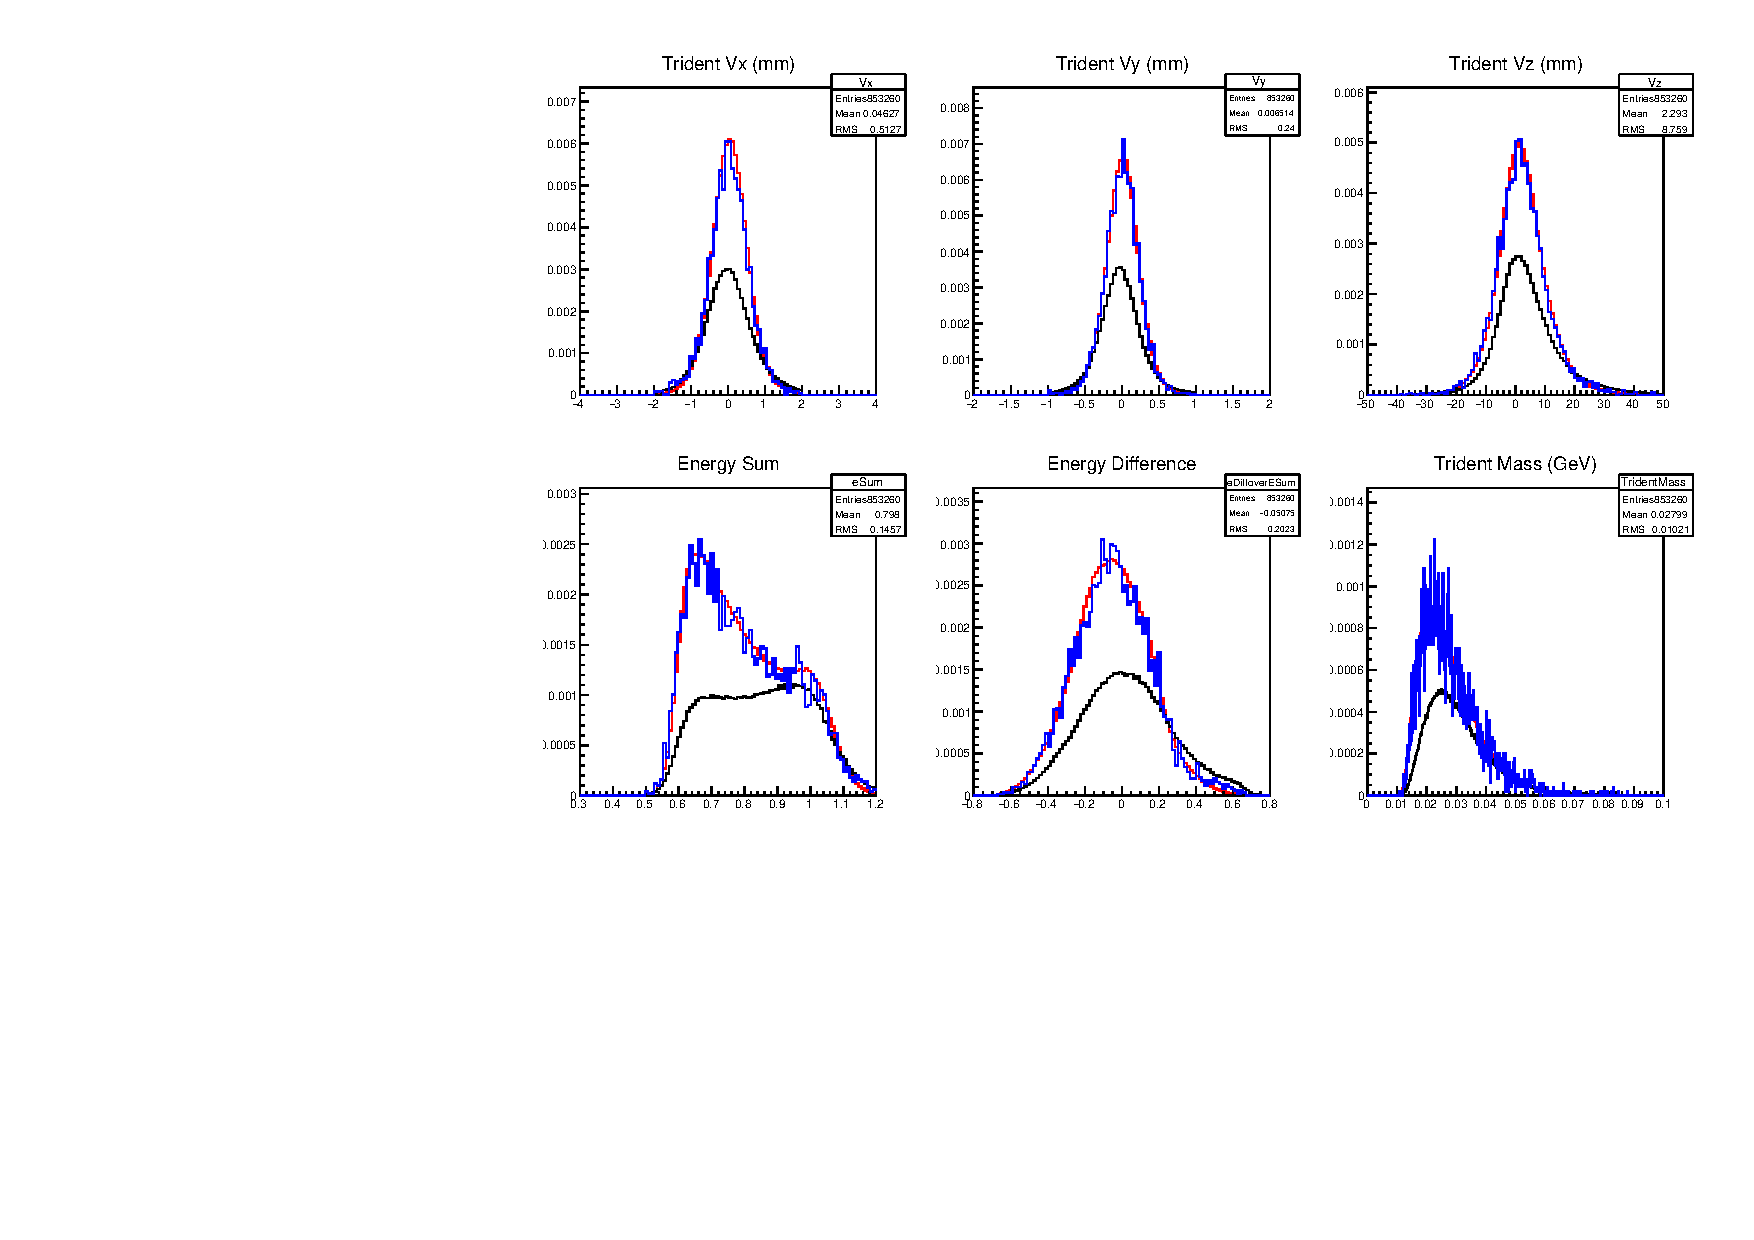
\includegraphics[width=0.9\textwidth]{v0summary-norm-to-XS.pdf}
  %%\caption{Make nicer plots!!!}
  %%\label{rfsignal}
%%\end{figure}	



\section{Conclusion}

Wrap it up

%----------------------------------------------------------------------------------------
%	REFERENCE LIST
%----------------------------------------------------------------------------------------

\begin{thebibliography}{99} % Bibliography - this is intentionally simple in this template
\end{thebibliography}

%----------------------------------------------------------------------------------------

%\end{multicols}

\end{document}
